\origsection{2}{建筑（The building）}
\origsubsection{2.1}{定义（Definitions）}
$G$ 在 $K$ 上的建筑（building）$\mathscr B=\mathscr B(G,K)$ 可将 $G$ 的各个极大 $K$ 分裂环面的公寓粘合起来构造。更确切地，下述陈述给出 $\mathscr B$ 的一个定义；其中“$G(K)$ 集”指带 $G(K)$ 左作用的集合。

设 $A=A(G,S,K)$ 如 1.2。则在唯一同构意义下，存在唯一的包含 $A$ 的 $G(K)$ 集 $\mathscr B$，具有下述性质：$\mathscr B=\bigcup_{g\in G(K)}gA$；群 $N(K)$ 保持 $A$，并通过 $\nu$ 在其上作用（见 1.2）；对每个仿射根 $\alpha$，1.4 的群 $X_\alpha$ 逐点固定半公寓 $A_\alpha=\alpha^{-1}([0,\infty))$。

（注意：建筑 $\mathscr B$ 的“典范性”与 $A$ 相同，见 1.2。）

证明大致如下。假设 $G$ 半单（这一步不损失问题的本质）。在承认 1.4.1 和 1.4.2 的条件下，正如 1.5 所解释，[8，7.4] 证明了 $\mathscr B$ 的存在。于是显然存在具有所给性质的“泛”$G(K)$ 集 $\overline{\mathscr B}$，它由直积 $G(K)\times A$ 对某个等价关系取商得到。$\overline{\mathscr B}$ 到 [8，7.4.2] 定义的建筑 $\mathscr I$ 的典范映射显然满射，它也为单射，因为容易验证，$\overline{\mathscr B}$ 的一个点的稳定子包含其在 $\mathscr I$ 中的像的稳定子。因此，$\mathscr I$ 满射到任意具有所需性质的 $G(K)$ 集 $\mathscr B$；利用 [8，7.3.4] 可证明，$A$ 的点在 $\mathscr B$ 中的稳定子不能比在 $\mathscr I$ 中更大，否则它与 $N(K)$ 的交会超过规定的 $N(K)$ 在 $A$ 上的作用所允许的范围。

集合 $gA$，$g\in G(K)$，称为建筑的公寓。公寓 $gA$ 可自然等同于极大分裂环面 $\prescript{g}{}{S}$ 对应的公寓。这给出 $\mathscr B$ 的公寓与 $G$ 的极大 $K$ 分裂环面之间的一一对应：事实上，$gA$ 是被 $\prescript{g}{}{S}(K)$ 保持的唯一公寓（[8，2.8.11] 的证明说明这一点），而确定 $\prescript{g}{}{S}$ 的 $\prescript{g}{}{N}(K)$ 是 $gA$ 在 $G(K)$ 中的稳定子。“在多数情形下”，$gA$ 还可刻画为单位群
\[
\prescript{g}{}{S}^\circ=\{s\in\prescript{g}{}{S}(K)\mid\omega(\chi(s))=0\text{ 对所有 }\chi\in X^*(\prescript{g}{}{S})\}
\]
在 $\mathscr B$ 中的不动点集，但这并不总成立（更精确的陈述见 3.6）。

还需注意，半公寓 $A_\alpha$（$\alpha\in\Phi_{\mathrm{af}}$）从来不是群 $X_\alpha$ 的不动点集。事实上，若按下文 2.3 赋予 $\mathscr B$ 度量，则存在常数 $c$，使对 $A_\alpha$ 中距墙 $\partial A_\alpha$ 的距离为 $d$ 的每个点 $x$，整个以 $x$ 为中心、半径为 $cd$ 的球均被 $X_\alpha$ 逐点固定（见 [8，7.4.33]）。

如果 $S_1$ 为 $G^\circ$ 的中心的极大分裂环面，$G_1,\ldots,G_m$ 为 $G^\circ$ 的近单因子（almost simple factors），则建筑 $\mathscr B$ 典范同构于各建筑 $\mathscr B(S_1,K)$（它是仿射空间）与 $\mathscr B(G_i,K)$，$i=1,\ldots,m$，的直积。如果 $G$ 在 $K$ 上各向异性，即 $S=\{1\}$，则 $\mathscr B$ 只有一个点。如果 $G=R_{L/K}H$，其中 $L/K$ 可分、$H$ 为 $L$ 上约化群，则建筑 $\mathscr B(G,K)$ 与 $\mathscr B(H,L)$ 典范同构。
\origsubsection{2.2}{建筑上的仿射结构、面、收缩、拓扑及其他典范结构（Affine structures, facets, retractions, topology and other canonical structures）}
由于 $A$ 在 $G(K)$ 中的稳定子 $N(K)$ 保持其仿射结构及分面的划分，$\mathscr B$ 的每个公寓 $gA$，$g\in G(K)$，都自然带有实仿射空间结构与分面的划分。这些结构在交集上一致。事实上，

\paragraph*{2.2.1.}若 $A',A''$ 为两个公寓，则存在 $G(K)$ 的元素，将 $A'$ 映至 $A''$，并逐点固定交集 $A'\cap A''$；此外，$A'\cap A''$ 是 $A'$ 中若干面的闭凸并集（因此在 $A''$ 中也是如此）[8，7.4.8]。

由此得到 $\mathscr B$ 的分面划分，其中在公寓中为开集的面称为室。特别地，如果 $G^\circ$ 拟单（半单），则 $\mathscr B$ 是单纯（多单纯）复形（simplicial/polysimplicial complex）。

给定 $\mathscr B$ 的两个面，存在同时包含它们的公寓 [8，7.4.18]。特别地，给定 $x,y\in\mathscr B$，存在包含它们的公寓。由 2.2.1，对 $t\in[0,1]\subset\R$，在这样的公寓中定义的点 $(1-t)x+ty$ 与公寓的选择无关。集合 $\{(1-t)x+ty\mid t\in[0,1]\}$ 称为 $\mathscr B$ 中连接 $x,y$ 的测地线段（geodesic segment）。

设 $A'$ 为一个公寓，$C\subset A'$ 为一个室。对每个包含 $C$ 的公寓，存在从该公寓到 $A'$ 的唯一逐点固定 $C$ 的仿射空间同构。由 2.2.1，这些同构可粘合成映射 $\rho_{A';C}:\mathscr B\to A'$，称为以 $C$ 为中心、从 $\mathscr B$ 到 $A'$ 的收缩（retraction）。显然，$\rho_{A';C}$ 将测地线段映为折线，即有限条测地线段的连通并。

通常在建筑 $\mathscr B$ 上赋予一个 $G(K)$ 不变拓扑，最自然的定义借助下文 2.3 的度量；也可更典范地定义为使所有 $\rho_{A';C}$ 连续的最弱拓扑。如果剩余域 $\overline K$ 有限，此拓扑使 $\mathscr B$ 成为局部紧空间，且与“CW 拓扑”一致，即全部公寓不交并上自然拓扑的商拓扑。否则，它严格弱于后者。无论何种情形，拓扑空间 $\mathscr B$ 均可缩（contractible）。事实上，对每个点 $x\in\mathscr B$，由 $\varphi_t(y)=tx+(1-t)y$ 定义的映射 $\varphi_t:\mathscr B\to\mathscr B$，构成从恒等映射到 $\mathscr B$ 至 $\{x\}$ 的收缩的同伦（homotopy）[8，7.4.20]。

如果 $\mathscr B$ 的一个子集在某个收缩 $\rho_{A';C}$ 下的像有界，则称其有界（bounded）；容易看出，此时它在每个这种收缩下的像均有界。按通常的定义，若对 $G$ 上每个 $K$ 正则函数 $f$，集合 $\omega(f(H))$ 都有下界，就称 $G(K)$ 的子集 $H$ 有界。$G(K)$ 在 $\mathscr B$ 上的作用在下述意义下有界且“适当”（proper）：映射 $(g,b)\mapsto(gb,b)$，从 $G(K)\times\mathscr B$ 到 $\mathscr B\times\mathscr B$，将有界子集（即有界集的乘积的子集）映为有界集，而且 $\mathscr B\times\mathscr B$ 中有界子集的原像有界。若 $\overline K$ 有限，“有界”与“相对紧”同义；特别地，$G(K)$ 在 $\mathscr B$ 上的作用在通常意义下适当。
\origsubsection{2.3}{度量与单纯形分解（Metric and simplicial decomposition）}
在各种问题中，建筑对于 $p$ 进约化群所起的作用，类似于对称空间（symmetric spaces）在非紧实单 Lie 群研究中所起的作用（见 [24，第 5 节] 及其中的参考文献）。本节说明这种类比的若干方面；另参见 [18，5.32]。注意，与 2.2 引入的结构不同，这里考虑的结构至少在 $G$ 不半单时并非典范。

在 $V$ 中选取一个 Weyl 群 $\prescript{v}{}{W}$ 不变的内积。如果 $G$ 拟单，此内积在差一个标量因子的意义下唯一，且有各种“自然”的正规化方法（Killing 型、规定短余根长度等）。$G$ 半单时，也可逐分支作典范选择；一般情形则不行。由该内积得到 $A$ 上的 Euclidean 距离，再通过 $G(K)$ 的作用得到任一公寓上的距离。由 2.2.1，$\mathscr B$ 的两点 $x,y$ 在包含它们的所有公寓中有相同距离 $d(x,y)$。2.2 中收缩 $\rho_{A';C}$ 的性质容易推出：赋予距离函数 $d:\mathscr B\times\mathscr B\to\R_+$ 后，建筑 $\mathscr B$ 是完备度量空间（complete metric space）[8，2.5]。对应拓扑与 2.2 定义的相同。再次利用收缩，可证明 [8，3.2.1]：若 $x,y,z,m\in\mathscr B$ 且 $d(x,m)=d(y,m)=\frac12d(x,y)$，则
\[
d(x,z)^2+d(y,z)^2\geq2d(m,z)^2+\tfrac12d(x,y)^2.
\]
在 Riemann 几何中，此不等式刻画截面曲率（sectional curvature）为负的空间（因而在非紧不可约对称空间中成立）。\footnote{\textbf{译者注（本次校订）：}这里应为截面曲率“非正”，而非“为负”。在完备、单连通的 Riemann 流形中，所示中点不等式对应非正曲率；高秩非紧对称空间包含二维平坦子空间，其截面曲率可以为零。}与 Riemann 情形类似，这里可用它证明下面的不动点定理。

\paragraph*{2.3.1.}$\mathscr B$ 的等距变换（isometries）的一个有界群必有不动点 [8，3.2.4]。有趣的应用来自 Galois 群（建筑的“Galois 下降”，Galois descent）及 $G(K)$ 的有界子群（见 3.2）。

某些应用中（例如 [2]），需要 $\mathscr B$ 的一个 $G(K)$ 不变单纯形分解。只需选取 $A$ 的一个 $N(K)$ 不变、比按面划分更细的单纯形分解（容易看出这种分解总存在），并通过 $G(K)$ 作用搬移到全部公寓。如果 $G$ 半单，可更直接地使用多单纯面划分的典范重心细分（barycentric subdivision）。如果 $G$ 拟单，该划分本身就满足要求。
\origsubsection{2.4}{Dynkin 图；特殊点与超特殊点（Dynkin diagram; special and hyperspecial points）}
设 $C$ 为 $\mathscr B$ 的一个室。从包含 $C$ 的任一公寓出发，可依 1.8 定义局部 Dynkin 图 $\Delta(G,C)$；由 2.2.1，它在唯一同构意义下与公寓选择无关。如果 $C'$ 为另一个室，将 1.8.1 用于同时包含 $C,C'$ 的任一公寓，得到同构 $\varphi_{C'C}:\Delta(G,C)\to\Delta(G,C')$，由 2.2.1，它仍与公寓无关。所有这些同构相容：若 $C,C',C''$ 为三个室，则 $\varphi_{C''C}=\varphi_{C''C'}\circ\varphi_{C'C}$。因此，可以谈论 $G$ 在 $K$ 上的局部 Dynkin 图 $\Delta(G)=\Delta(G,K)$，它在唯一同构意义下良定义。绝对局部 Dynkin 图（1.11）、局部指标（1.11）亦然；前者正是 $G$ 在 $K$ 的非分歧闭包 $K_1$ 上的图 $\Delta(G,K_1)$。

1.9 和 1.10 的定义立即推广至建筑 $\mathscr B$ 的任意点 $x$、任意面 $F$：选取包含 $x$ 或 $F$ 的公寓，采用相应定义，再由 2.2.1 得到结果与公寓选择无关。因此，$\mathscr B$ 的每个点 $x$（面 $F$）都典范地对应于 $\Delta(G)$ 的一个顶点集 $I_x$（$I_F$），以及根系 $\Phi_x$（$\Phi_F$）；后者仅在非典范同构意义下定义。也可谈论 $\mathscr B$ 的特殊点与超特殊点。1.9 最后一段用 $I_x$ 判别特殊点的准则当然仍成立。超特殊点存在的必要条件是 $G$ 在 $K$ 的某个非分歧扩张上分裂；若 $G$ 拟分裂，这一条件也充分。

图 $\Delta(G)$ 的每个顶点 $v$ 都带一个整数 $d(v)$。1.8 中的定义借助公寓 $A$，但仍由 2.2.1，结果与其选择无关。如果剩余域 $\overline K$ 有限，同构于 $\F_q$，则 $d(v)$ 可解释如下：“类型为 $v$”的余维一的面 $F$，即 $I_F$ 为 $\Delta(G)$ 全部顶点集去掉 $v$ 后的补集，恰被 $q^{d(v)}+1$ 个室的闭包包含（见 3.5）。
\origsubsection{2.5}{自同构的作用；特殊点与超特殊点的共轭类（Action of automorphisms; conjugacy classes of special and hyperspecial points）}
$G$ 的全部 $K$ 自同构组成的群 $(\Aut G)(K)$，特别是 $G^\circ$ 的伴随群 $G_{\mathrm{ad}}$ 的有理点群 $G_{\mathrm{ad}}(K)$，通过结构搬移作用于 $\mathscr B$ 与局部 Dynkin 图 $\Delta=\Delta(G)$。通过典范同态 $\operatorname{int}:G\to\Aut G$，得到 $G(K)$ 在 $\mathscr B$ 与 $\Delta$ 上的作用。由 $\mathscr B$ 作为 $G(K)$ 集的定义所给出的 $G(K)$ 在 $\mathscr B$ 上的作用，在 $G$ 半单时与此作用一致，一般时不然；但两者在 $\Delta$ 上诱导的作用总相同。记 $\Xi=\Xi(G,K)$ 为 $G(K)$ 在 $\Aut\Delta$ 中的像。

如果 $G$ 半单且单连通，它在 $\Delta$ 上的作用平凡，即 $\Xi=\{1\}$（这是 1.13 所述现象的又一体现）。

假设 $G$ 连通。则 $\Xi$ 也是 $Z(K)$ 在 $\Aut\Delta$ 中的像，计算如下：以 $\widetilde G$ 表示 $G$ 导群的单连通覆盖，以 $\widetilde S$ 表示 $\widetilde G$ 中其在 $G$ 中的像包含于 $S$ 的极大分裂环面，以 $\widetilde Z$ 表示 $\widetilde S$ 在 $\widetilde G$ 中的中心化子，以 $S_1$ 表示 $S$ 中在 $G$ 内中心的极大子环面，以 $Z_s$ 表示 $\widetilde Z(K)$ 在 $Z(K)$ 中的像。则 $S_1(K)$、$Z_s$ 以及 $Z_c=\{z\in Z(K)\mid\omega(\chi(z))=0\text{ 对所有 }\chi\in X^*(Z)\}$（见 1.2）均为 $Z(K)$ 的正规子群，乘积 $S_1(K)Z_sZ_c$ 是 $Z(K)$ 在 $\Delta$ 上作用的核。因此
\[
\Xi=Z(K)/(S_1(K)\cdot Z_s\cdot Z_c).
\]
若 $G$ 拟分裂，特别是 $\overline K$ 代数闭时，$Z,\widetilde Z$ 是环面，计算 $\Xi$ 尤为简单。注意，在多数常见情形中，$\Aut\Delta$ 的子群 $\Xi$ 由其底层“抽象”群唯一确定。

$\mathscr B$ 的两个面 $F,F'$ 位于同一个 $G(K)$ 轨道中（对上述两种 $G(K)$ 作用均如此），当且仅当 $I_F,I_{F'}$（见 2.4）位于同一个 $\Xi$ 轨道。特别地，若 $G$ 半单且单连通，则 $G(K)$ 在 $\mathscr B$ 的特殊点集中的轨道，与从 $\Delta$ 每个连通分支各取一个特殊顶点所成的顶点集，典范地一一对应。

假设 $G$ 半单。若 $G$ 在 $K$ 上分裂，则 $G_{\mathrm{ad}}(K)$ 传递地置换 $\mathscr B$ 的特殊点，这是 [5，VI.2.2，命题 2] 的直接推论。逐情形分析表明，对任意半单 $G$，$G_{\mathrm{ad}}(K)$ 都传递地置换特殊点；可能的例外只在 $\Delta$ 的底层 Coxeter 图存在形如下图的连通分支时：
\begin{center}
\begin{tikzpicture}[x=.6cm,y=.6cm]
\draw(0,.07)--(1,.07) (0,-.07)--(1,-.07) (1,0)--(2,0);\draw[dashed](2,0)--(3,0);\draw(3,0)--(4,0) (4,.07)--(5,.07) (4,-.07)--(5,-.07);
\foreach \x in {0,1,2,3,4,5}{\draw(\x,-.1)--(\x,.1);}
\node[above]at(0,.15){s};\node[above]at(5,.15){s};\node at(6,0){或};\draw[line width=2pt](7,0)--(8,0);\node[above]at(7,.15){s};\node[above]at(8,.15){s};
\end{tikzpicture}
\end{center}
现假设 $G$ 拟单，且上述 Coxeter 图是这些图之一。$G_{\mathrm{ad}}(K)$（甚至 $(\Aut G)(K)$）传递地置换特殊点的显然必要条件，是存在置换其两个特殊顶点的 $\Delta$ 自同构，且它们所带的 $d(v)$ 相等。可验证，若剩余域 $\overline K$ 有限，这些条件也充分。

对任意 $G$，若 $\mathscr B$ 有超特殊点，则由这种点构成的面被 $G_{\mathrm{ad}}(K)$ 传递地置换；因而 $G$ 半单时，这些点本身被传递地置换。
\origsubsection{2.6}{域扩张下的行为（Behaviour under field extensions）}
建筑关于 Galois 扩张具有函子性。

更确切地，对 $K$ 的每个 Galois 扩张 $K_1$，可考虑建筑 $\mathscr B(G,K_1)$，Galois 群 $\Gal(K_1/K)$ 在其上自然作用（非半单情形须按 1.2 使公寓、从而使 $\mathscr B$ 典范化）。存在唯一的单射系统
\[
\iota_{K_2K_1}:\mathscr B(G,K_1)\longrightarrow\mathscr B(G,K_2),
\qquad K_1\subset K_2,\quad K_1,K_2\text{ 为 }K\text{ 的 Galois 扩张},
\]
满足：$\iota_{K_2K_1}$ 的像被 $\Gal(K_2/K_1)$ 逐点固定；$\iota_{K_2K_1}$ 在 $\mathscr B(G,K_1)$ 的任一公寓上的限制，是映入 $\mathscr B(G,K_2)$ 的某个公寓的仿射映射；$\iota_{K_2K_1}$ 是 $G(K_1)$ 等变的（covariant）；若 $K_1\subset K_2\subset K_3$，则 $\iota_{K_3K_1}=\iota_{K_3K_2}\circ\iota_{K_2K_1}$。最后一个性质使我们能相容地将每个 $\mathscr B(G,K_1)$ 与它在每个 $\iota_{K_2K_1}$ 下的像等同。

\paragraph*{2.6.1.}若 $K_1/K$ 非分歧（甚至驯分歧，见 [19]），则 $\mathscr B$ 是 $\Gal(K_1/K)$ 在 $\mathscr B(G,K_1)$ 中的不动点集；公寓 $A=A(G,S,K)$ 是 $\mathscr B$ 与任一包含 $S$ 的极大 $K_1$ 分裂 $K$ 环面 $S_1$ 的公寓 $A(G,S_1,K_1)$ 的交。仍假设 $K_1/K$ 非分歧，由 1.10.2，$\mathscr B$ 中在 $\mathscr B(G,K_1)$ 内特殊的点 $x$，在 $\mathscr B$ 中也特殊；若进一步 $G$ 在 $K_1$ 上分裂，则 $x$ 超特殊。

若 $K_1/K$ 野分歧（wildly ramified），$\Gal(K_1/K)$ 在 $\mathscr B(G,K_1)$ 中的不动点集可能严格大于 $\mathscr B$，其形状仿佛是在建筑 $\mathscr B$ 周围多长出了一些分支。例如，设 $G$ 分裂且不是环面，$K=\Q_2$，$K_1/K$ 完全分歧且 $K_1\ne K$（这蕴涵 $K_1/K$ 野分歧）。$\mathscr B$ 的公寓 $A=A(G,S,K)$ 也是 $\mathscr B(G,K_1)$ 的一个公寓。取 $A$ 中相对于 $K_1$ 的余维一的面 $F$，使它不是相对于 $K$ 的面（见 1.10.1 后的例子）。由 1.8 和 2.4 的最后断言，$\mathscr B(G,K_1)$ 中恰有一个不包含于 $A$、闭包包含 $F$ 的室；它当然被 $\Gal(K_1/K)$ 固定，且不可能包含于 $\mathscr B$，因为 $F$ 不是 $\mathscr B$ 的面。

上述结果的证明及更详细的分析见 [19]。
\origsubsection{2.7}{例：相对秩为一的群（Example: groups of relative rank 1）}
相对秩为一的半单群的建筑是维数为一的可缩单纯复形，即一棵树（tree）。它的全部顶点均为特殊点。如果 $\overline K\simeq\F_q$，$d,d'$ 为 Dynkin 图的两个顶点所带的整数 $d(v)$，则树的每条边的一个顶点的度为 $q^d+1$，另一个顶点的度为 $q^{d'}+1$（见 2.4）。例如，取 $\Q_2$ 上五个变量的一个非分裂二次型的特殊正交群，此时 $d=1$、$d'=2$，其建筑如图所示。此时度为 $5$ 的顶点超特殊，其余顶点不是。\footnote{\textbf{译者注（本次校订）：}对这里的非分裂五维二次型，最后一句中的“超特殊”不成立。它的特殊正交群是分裂 $\operatorname{SO}_5$ 的非拟分裂内形式；有限剩余域上，具有超特殊点的约化群必为拟分裂群。此例的顶点均为特殊点，但均非超特殊点，度数差异本身不能判定超特殊性。}
\begin{center}\begin{tikzpicture}[line width=.4pt,scale=1.1]
\coordinate (o)at(0,0);
\foreach \a in {90,210,330}{
\coordinate(a\a)at(\a:1);\draw(o)--(a\a);
\foreach \b in {-45,-15,15,45}{
\pgfmathsetmacro{\ang}{\a+\b}
\coordinate(b\a\b)at($(a\a)+(\ang:.62)$);\draw(a\a)--(b\a\b);
\foreach \c in {-16,16}{\pgfmathsetmacro{\angtwo}{\ang+\c}\coordinate(c\a\b\c)at($(b\a\b)+(\angtwo:.35)$);\draw(b\a\b)--(c\a\b\c);
\foreach \d in {-24,-8,8,24}{\pgfmathsetmacro{\angthree}{\angtwo+\d}\draw[densely dotted](c\a\b\c)--++(\angthree:.22);}
}
}
}
\end{tikzpicture}
\end{center}
\origsubsection{2.8}{例：$\SL_3$ 与 $\GL_3$（Example: $\SL_3$ and $\GL_3$）}
假设 $G=\SL_3$。建筑 $\mathscr B=\mathscr B(G,K)$ 是二维单纯复形，对 2.3 引入的度量，其极大单纯形是等边三角形。公寓为按熟知方式剖分成三角形的 Euclidean 平面：
\begin{center}
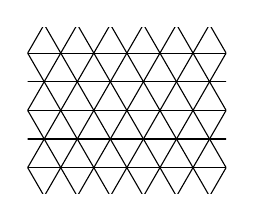
\begin{tikzpicture}[scale=.42]
\clip(-3,-2.5)rectangle(3,2.5);
\foreach \k in {-6,...,6}{\draw(-6,{.8660254*\k})--(6,{.8660254*\k});\draw({\k-3},-5.196152)--({\k+3},5.196152);\draw({\k+3},-5.196152)--({\k-3},5.196152);}
\end{tikzpicture}
\end{center}
整个建筑则沿每条边分叉；若 $q=\operatorname{card}\overline K$，则每条边属于 $q+1$ 个三角形。$\mathscr B$ 每个顶点的链环（link），是 $\SL_3(\overline K)$ 的“球面建筑”（spherical building），即 $\overline K$ 上某射影平面的“旗复形”（flag complex）；$\overline K\simeq\F_2$ 的特殊情形的图见 [24] 或 [26]。$\mathscr B$ 的全部顶点均超特殊。

建筑 $\mathscr B(\GL_3,K)$ 是 $\mathscr B$ 与一条仿射直线的直积。
\origsubsection{2.9}{例：一般线性群（Example: general linear groups）}
采用 1.14 的假设与记号。特别地，$D$ 为 $K$ 上的有限维中心除代数，$G=\GL_{n,D}$（所以 $G(K)=\GL_n(D)$）。则建筑 $\mathscr B=\mathscr B(G,K)$ 可解释为 $D^n$ 上全部“加性范数”（additive norms）的集合 $\mathcal N$，即所有满足
\[
\begin{aligned}
\varphi(x+y)&\geq\inf\{\varphi(x),\varphi(y)\},&&x,y\in D^n,\\
\varphi(xd)&=\varphi(x)+\omega(d),&&x\in D^n,\ d\in D
\end{aligned}
\]
的函数 $\varphi:D^n\to\R\cup\{+\infty\}$。\footnote{\textbf{译者注（本次校订）：}加性范数还须满足 $\varphi(x)=+\infty$ 当且仅当 $x=0$。仅靠上列两条关系，恒等于 $+\infty$ 的函数也会被纳入，而它不对应建筑中的点。}

更确切地，如 1.14 将公寓 $A$ 与 $V$ 等同，则将 $\sum_{i=1}^nv_ie_i$ 映为范数
\[
(x_1,\ldots,x_n)\longmapsto\inf\{\omega(x_i)-v_i\mid i=1,\ldots,n\}
\]
的映射 $A\to\mathcal N$，可唯一延拓为 $G(K)$ 集的同构 $\mathscr B\to\mathcal N$，其中 $G(K)$ 通过 $(g\varphi)(x)=\varphi(g^{-1}x)$ 作用于 $\mathcal N$。范数 $\varphi$ 特殊，即对应于 $\mathscr B$ 的特殊点，当且仅当存在向量空间 $D^n$ 的一组基 $(b_i)_{1\leq i\leq n}$ 及实数 $f$，使
\[
\varphi\left(\sum_{i=1}^nb_id_i\right)=f+\inf\{\omega(d_i)\mid i=1,\ldots,n\},\qquad d_i\in D.
\]
$\varphi$ 超特殊，当且仅当它特殊且 $D=K$。

$\mathscr B(\SL_{n,D},K)$ 的类似解释见 [8，第 238 页]。空间 $\mathcal N$ 最早由 O. Goldman 与 N. Iwahori [12] 考虑。
\origsubsection{2.10}{例：特殊酉群（Example: special unitary groups）}
$L,\omega,\pi_1,\Gamma_1,\tau,\delta$ 的含义同 1.15。特别地，$L/K$ 为可分二次扩张，且 $\delta=\sup\{\omega(d)\mid d\in L,d+d^\tau=1\}$。设 $E$ 为带有关于 $\tau$ 的非退化 Hermite 型 $h$ 的有限维 $L$ 向量空间，$G=\operatorname{SU}(h)$。则 $G$ 在 $K$ 上的建筑 $\mathscr B$（这也就是 $U(h)$ 的建筑），可解释为全部满足不等式
\[
\begin{aligned}
\omega(h(x,x))&\geq2\varphi(x)-\delta,&&x\in E,\\
\omega(h(x,y))&\geq\varphi(x)+\varphi(y),&&x,y\in E,
\end{aligned}
\]
且在逐点比较的偏序下为极大的加性范数 $\varphi:E\to\R\cup\{+\infty\}$ 的集合 $\mathcal N_h$（更一般的结果见 [8，第 239 页]）。

再假设 $E=L^{2n+1}$，且 $h$ 如 1.15（1）。$\mathscr B$ 与 $\mathcal N_h$ 的等同可更具体地描述：沿用 1.15 的记号，将 $\sum_{i=1}^nv_ie_i$ 映为范数\nobreak\footnote{\textbf{译者注（本次校订）：}本节两处显式范数中的中间坐标项应为 $\omega(x_0)+\delta/2$，而非 $\omega(x_0)-\delta$。取 $x=b_0$，则 $h(b_0,b_0)=1$，上面的第一条不等式给出 $\varphi(b_0)\le\delta/2$，极大范数取等号；原式在 $\delta<0$ 时已经违反该不等式。另外，式2.10(1)左边的求和应遍历 $-n\le i\le n$，以包括负指标和零指标。}
\[
(x_{-n},\ldots,x_n)\longmapsto
\inf\{\omega(x_i)-v_i,\omega(x_{-i})+v_i,\omega(x_0)-\delta\mid1\leq i\leq n\}
\]
的映射 $A\to\mathcal N_h$，唯一延拓为 $G(K)$ 集的同构 $\mathscr B\to\mathcal N_h$。范数 $\varphi\in\mathcal N_h$ 特殊，即对应 $\mathscr B$ 的特殊点，当且仅当存在 $E$ 的一组基 $(b_i)$，使 $h$ 关于此基为 1.15（1）的形式，且存在常数 $f\in\frac12\Gamma_1$，使对 $x_i\in L$，有
\[
\varphi\left(\sum_{i=1}^nb_ix_i\right)=
\inf\{\omega(x_i)-f,\omega(x_{-i})+f,\omega(x_0)-\delta\mid1\leq i\leq n\}.\tag{2.10(1)}
\]
这时可选基 $(b_i)$ 使 $f=0$ 或 $\frac12\omega(\pi_1)$。若 $L/K$ 非分歧且存在 $E$ 的基 $(b_i)$，使（1）在 $f=0$ 时成立，则范数 $\varphi$ 超特殊。
